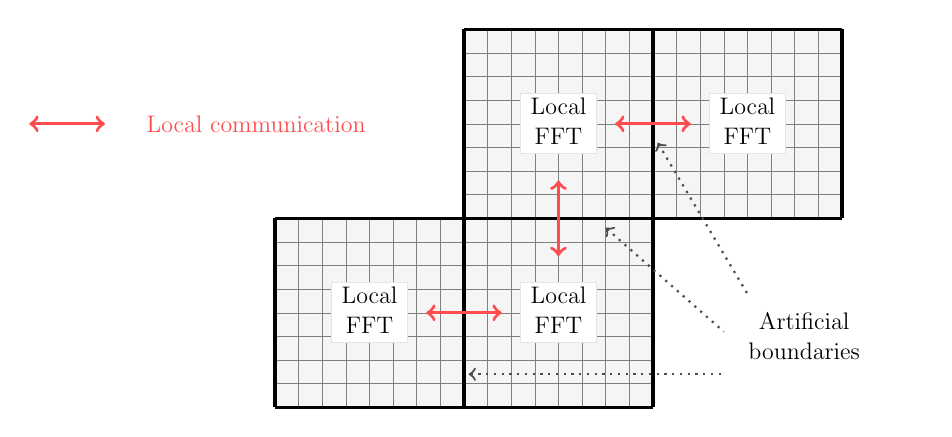
\begin{tikzpicture}
[
scale=0.6,
every node/.style={scale=0.6},
Background/.style={rectangle,draw=black!04,fill=black!04, thin, minimum size = 4 cm},
Obstruction/.style={rectangle,draw=black!70,fill=black!40, very thick, minimum size=1cm},
Finegrid/.style={step=0.5cm,gray,very thin},
Thickline/.style={-,draw=black!100,fill=black!02, very thick},
Thinline/.style={draw=black!100,fill=black!02, very thin},
Ball/.style={circle, draw=black!40, fill=red!20, thin, minimum size=3.5mm},
Circle/.style={circle,draw=black!40,fill=black!06,thin,minimum size=35.5mm},
Rectangle/.style={rectangle,draw=black!10,fill=white,inner xsep=0pt, inner ysep=0pt,},
Box/.style= {very thin, rectangle, inner xsep=10pt, inner ysep=10pt,},
ComArrow/.style= {<->,very thick, draw=red!70,},
DotArrow/.style= {<-, thick, dotted, draw=black!70,},
]

\node[Background] at (  2,2) {};
\node[Background] at (  6,2) {};
\node[Background] at (  6,6) {};
\node[Background] at (10,6) {};

\node[Obstruction] at (2,2) {};

\draw[Finegrid] (0,0) grid (  8,4);
\draw[Finegrid] (4,4) grid (12,8);

\draw[Thickline] (0,0)--(  8,0);
\draw[Thickline] (4,8)--(12,8);
\draw[Thickline] (0,4)--(  4,4);
\draw[Thickline] (8,4)--(12,4);

\draw[Thickline] (  0,0)--(  0,4);
\draw[Thickline] (  4,8)--(12,8);
\draw[Thickline] (  4,4)--(  4,8);
\draw[Thickline] (  8,0)--(  8,4);
\draw[Thickline] (12,4)--(12,8);

\draw[Thickline] (4,0)--(4,4);
\draw[Thickline] (4,4)--(8,4);
\draw[Thickline] (8,4)--(8,8);

\node[Rectangle] at (  2,2.0) {\Large \begin{tabular}{c} Local \\ FFT\end{tabular}};
\node[Rectangle] at (  6,2.0) {\Large \begin{tabular}{c} Local \\ FFT\end{tabular}};
\node[Rectangle] at (  6,6.0) {\Large \begin{tabular}{c} Local \\ FFT\end{tabular}};
\node[Rectangle] at (10,6.0) {\Large \begin{tabular}{c} Local \\ FFT\end{tabular}};

\draw[ComArrow](3.2,2)--(4.8,2);
\draw[ComArrow](6,3.2)--(6,4.8);
\draw[ComArrow](7.2,6)--(8.8,6);

\draw [DotArrow] (8.1,5.6) -- (10.0,2.4);
\draw [DotArrow] (7.0,3.8) -- (  9.5,1.6);
\draw [DotArrow] (4.1,0.7) -- (  9.5,0.7);

\node [Box] (box) at (11.2,1.5){%
    \begin{minipage}{0.36\textwidth}
    \begin{center}
        {\Large Artificial \\[1ex]
           boundaries}
    \end{center}
    \end{minipage}};

\draw[ComArrow](-5.2,6)--(-3.6,6);
\node [Box,red!70] (box) at (-0.4,6){%
    \begin{minipage}{0.56\textwidth}
    \begin{center}
        {\Large Local communication}
    \end{center}
    \end{minipage}};

\end{tikzpicture}
